\documentclass[12pt, twoside]{article}
\usepackage[letterpaper, margin=1in, headsep=0.5in]{geometry}
\usepackage[english]{babel}
\usepackage[utf8]{inputenc}
\usepackage{amsmath}
\usepackage{amsfonts}
\usepackage{amssymb}
\usepackage{tikz}
%\usetikzlibrary{quotes, angles}

\usepackage{graphicx}
\usepackage{enumitem}
\usepackage{multicol}

\usepackage{fancyhdr}
\pagestyle{fancy}
\fancyhf{}
\renewcommand{\headrulewidth}{0pt} % disable the underline of the header

\fancyhead[RE]{\thepage}
\fancyhead[RO]{\thepage \\ Name: \hspace{3cm}}
\fancyhead[L]{BECA / Dr. Huson / 10.3 Geometry\\* 14 January 2019}

\begin{document}
\subsubsection*{Do Now}
For graphs, use a pencil and straight edge. Label each line.
  \begin{enumerate}

\item Solve for $y$, then graph the two inequalities.

  \begin{multicols}{2}
    $-3y + 6 < x$ \\
    $2x - 2y \geq 8$
  \end{multicols}
  \vspace{2.5cm}

  \begin{center} %4 quadrant regents grid w T-Chart
  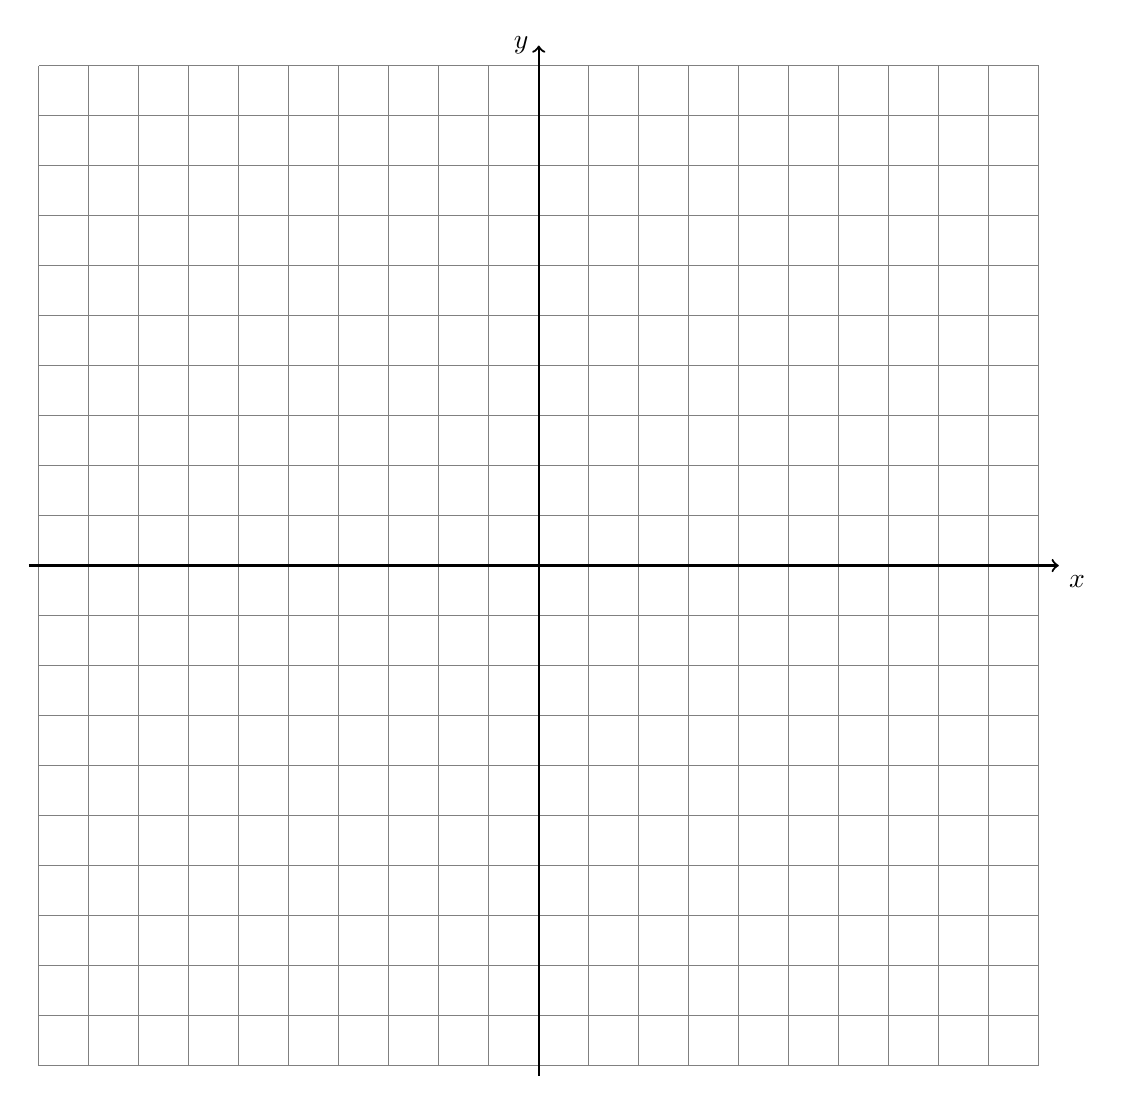
\begin{tikzpicture}[scale=.635]
    \draw [help lines] (-10,-10) grid (10,10);
    \draw [thick, ->] (-10.2,0) -- (10.4,0) node [below right] {$x$};
    \draw [thick, ->] (0,-10.2)--(0,10.4) node [left] {$y$};
  \end{tikzpicture}
  \end{center}

  Mark the solution set with a capital ``S". Is the point written on the board a solution? Justify your answer.

  \newpage

  \subsubsection*{Fractional Algebra}
      \item $\dfrac{7}{4}(2x + 4) = 14$ \vspace{3cm}
      \item $\dfrac{3}{x}(7x - 9) = 12$ \vspace{3cm}

  \subsection*{Quadratic Formula}
      \item Solve $x^2 - 3x - 10$ by factoring. Then check with the quadratic formula. \vspace{3cm}
      \item Solve $x^2 + 7x  - 17$.

\end{document}
